\documentclass[a4paper]{report}

\author{Misrraim~Su\'arez~P\'erez}
\title{FirstMarket}

\usepackage{comment}
\usepackage[utf8]{inputenc}

\usepackage{csquotes}

\usepackage{graphicx}
\graphicspath{ {./images/} }



\begin{document}

    \maketitle
    \tableofcontents

    % INTRODUCCION
    \section{Introducción}
    El presente proyecto se enmarca dentro del Proyecto Final de Grado correspondiente al Grado en Ingeniería Informática
    de la Universidad Nacional de Educación a Distancia.

    Se basa en el proyecto específico ofertado por el Departamento de Sistemas de Comunicación y Control de la UNED titulado \emph{Desarrollo de un portal de comercio electrónico}.
    Citando la propia descripción de dicha oferta de proyecto específico:
    \begin{displayquote}
        El proyecto consiste en el desarrollo de un portal web orientado al comercio electrónico.
        Dicha aplicación permitirá al comprador seleccionar artículos, realizar pedidos y pagos a través de una pasarela.
        El sistema también ofrecerá al comerciante gestionar los artículos expuestos en el portal.
    \end{displayquote}


    \subsection{Motivación y Objetivos}
    Desde un primer momento la intención fue desarrollar un proyecto que tuviese la mayor proyección posible en el mercado laboral, lo que,
    junto con un fuerte interés personal hacia el ecosistema de internet, llevó a la decisión de escoger esta propuesta.

    La idea era desarrollar algo moderno, útil, con reflejo real en la sociedad y que, como se ha dicho, cumpliese el papel de facilitar la inserción laboral.

    En este sentido, las aplicaciones web en general, y las específicas de comercio electrónico en particular, cumplen a la perfección los requisitos comentados.
    A nadie se le escapa hoy en día la implantación casi ubicua que estas tecnologías tienen en la sociedad.

    Por otro lado, y en clara conexión con lo comentado, otro objetivo de este último trabajo del plan de estudios fue el de servir como \emph{compensador} final de carencias formativas.
    En este sentido, el control de versiones con Git era una tarea pendiente inaplazable, así como profundizar en tecnologías web básicas como HTTP, HTML, CSS ó JavaScript.
    Además, ampliar el dominio de las tecnologías Java siempre fue algo muy deseable.

    Conviene no dejar de lado, por obvio, que un objetivo fundamental del presente trabajo es el de dar fin al plan de estudios.
    Remarcar esto es relevante porque en múltiples situaciones puede entrar en conflicto con la intención de desarrollar una aplicación web lo más moderna posible.
    Como se explicará más adelante en esta memoria, el mundo de las tecnologías web es muy cambiante,
    y pretender desarrollar una aplicación web alineada con el estado del arte en la materia partiendo, como es el caso, desde prácticamente cero conocimientos,
    sale fuera del marco de un trabajo de estas características.

    Por tanto, siempre se ha tenido en cuenta un compromiso entre recursos disponibles (principalmente tiempo y conocimientos) y grado de modernidad en las tecnologías usadas.

    En definitiva, el principio fundamental que ha guiado la toma de decisión ha sido el reforzar, y alinear en la medida de lo posible con el estado del arte,las habilidades técnicas fruto del plan de estudios, de forma a facilitar una futura integración en la industria web,
    a la par de satisfacer una histórica inquietud personal en la materia.


    \subsection{Internet, Web y Aplicaciones Web}
    En esta sección se pretende ofrecer una pequeña descripción que establezca el contexto en el que situar la aplicación web desarrollada.

    \subsubsection{¿Qué es Internet?}
    Tal como se explica en [computer-networking], esta pregunta puede ser respondida desde dos puntos de vista complementarios.

    Por un lado, desde una perspectiva \textbf{hardware}, Internet es una red que conecta miles de millones de dispositivos en todo el mundo,
    denominados \emph{hosts} o \emph{sistemas finales}, por medio de \emph{enlaces de comunicación} y \emph{conmutadores de paquetes}.
    
    Los enlaces de comunicación son diferentes tipos de medios físicos que transfieren ondas electromagnéticas. Así, puede tratarse de medios guiados, como cables de cobre, cables coaxiales o fibra óptica, o no guiados, como el espectro de radio.
    
    Cuando un sistema final decide enviar información a otro sistema final, el emisor fragmenta los datos en \emph{paquetes} de información y los envía al destinatario a través de la red. Una vez en destino, el sistema final receptor ensambla los paquetes para reconstruir los datos originales.

    Un conmutador de paquetes toma un paquete que llega a uno de sus enlaces de comunicación entrantes y lo reenvía a uno de sus enlaces de comunicación salientes.

    Estas \emph{redes de conmutación de paquetes} se pueden entender de forma análoga a una empresa que necesita mover una gran cantidad de carga entre dos almacenes separados gran distancia. En el almacén de origen la carga se divide y organiza en diferentes contenedores. Cada uno de los contenedores viaja de forma independiente a través de la red de transporte disponible siguiendo posiblemente rutas no del todo iguales. Por ejemplo, unos contenedores pueden ir por ciertas carreteras en ciertos camiones mientras que otros pueden viajar en tren o incluso en barco, o cualquier combinación de los anteriores. Lo importante es la independencia entre la ruta de un contenedor concreto con los demás. Una vez llegados al almacén de destino, la carga se extrae de los contenedores y se agrupa con el resto que llega del mismo envío.
    
    Así, los paquetes son análogos a los contenedores, los enlaces de comunicación son análogos a las vías de transporte, los conmutadores de paquetes son análogos a las intersecciones o discontinuidades en las vías de transporte (piénsese en una simple rotonda), y los sistemas finales son análogos a los almacenes. Pues bien, de igual forma que un contenedor toma un camino a través de la red de transporte, un paquete de información toma un camino a través de la infraestructura de Internet.

    Por otro lado, es posible describir Internet desde un punto de vista \textbf{software} como un servicio a las aplicaciones distribuidas. Se dice que las aplicaciones son aplicaciones distribuidas, o \textbf{aplicaciones de Internet}, cuando se ejecutan en diferentes máquinas que intercambian datos entre sí. Es importante destacar que las aplicaciones de Internet se ejecutan estrictamente en los sistemas finales, no en la infraestructura de la red, que es agnóstica (o debiera serlo) de la semántica de la información que está trasportando.
    
    Así, puede pensarse en Internet como un servicio postal, que garantiza el envío de información entre partes, las cuales pueden estar desarrollando cualquier tipo de actividad basada, entre otras cosas, en la propia comunicación que mantienen.
    
    \subsubsection{¿Qué es la World Wide Web?}
    
    \subsubsection{¿Qué es una Aplicación Web?}

    \subsection{Estructura de la Memoria}
    Estructura

    % ANALISIS
    \section{Análisis}

        \subsection{Requisitos}

            La aplicaci\'on debe admitir los roles y capacidades siguientes:
            \begin{enumerate}
                \item Usuario an\'onimo (UA).
                \begin{itemize}
                    \item Por defecto, al acceder al sitio web se hace como UA, sin ninguna validacion ni credencial. Basta con acceder a la pagina (url) de inicio de la aplicacion.
                    \item Un UA debe poder realizar b\'usquedas de libros, es decir, debe tener pleno acceso a la exploracion del cat\'alogo.
                    \item La plena exploraci\'on del cat\'alogo debe permitir realizar b\'usque\-das filtradas seg\'un 0, 1 o m\'as criterios, tales como: categor\'\i{}a, t\'\i{}tulo o autor.
                    \item Un UA debe poder visualizar informacion detallada de un libro, por ejemplo de entre los obtenidos tras una busqueda.
                    \item Un UA debe poder consultar las promociones disponibles.
                    \item Un UA debe poder registrarse en el sistema completando un formulario (nombre, contrase\~na, direccion de correo electronico, etc.).
                    \item finalizado el proceso de registro, el nuevo UR debe recibir confirmacion por e-mail
                    \item en su caso, un UA debe poder hacer login en el sistema.
                    \item en su caso, un UA debe poder realizar el procedimiento de recuperacion de contrase\~na.
                \end{itemize}
                \item Usuario registrado (UR). Este perfil representa a un usuario que ha pasado de an\'onimo a registrado. Un UR posee todas las capacidades del UA, m\'as otras espec\'\i{}ficas suyas, a saber:
                \begin{itemize}
                    \item Poder editar la informacion de su perfil de usuario.
                    \item Realizar pedidos y efectuar los correspondientes pagos a traves de una pasarela segura.
                    \item Disponer de un carrito virtual para la gestion de la compra.
                    \item En el carrito se debe poder introducir, modificar la cantidad o eliminar libros (esto ultimo de uno en uno o todos a la vez).
                    \item en cualquier momento del proceso de realizar un pedido, el UR debe poder cancelarlo
                    \item Tras una compra, el UR debe recibir confirmacion en su correo electronico
                    \item un UR debe poder consultar el estado de sus pedidos
                    \item Puntuar (de alguna manera, p.e. estrellas del 1 al 5) un determinado libro que haya adquirido. Debe poder hacerlo en cualquier momento tras la compra.
                    \item Consultar un historico de sus transacciones, detallando los libros comprados, la fecha de la compra y el precio de cada uno.
                    \item Darse de baja como UR.
                    \item Cerrar sesion.
                    \item Un UR debe poder ponerse en contacto con el admin a traves de un formulario de contacto, recibiendo confirmacion por e-mail tras el envio del mismo.
                \end{itemize}
                \item Usuario Administrador
                \begin{itemize}
                    \item Ver y editar (a\~nadir, modificar, eliminar) la jerarquia de categorias (CRUD categorias).
                    \item Ver y editar (a\~nadir, modificar, eliminar) la informacion relativa a los libros (titulo, autor/es, editorial, precio, disponibilidad, \ldots) (CRUD libros).
                    \item Crear, modificar o eliminar promociones de libros (CRUD promos).
                    \item Tener acceso a la informacion de los UR, salvo sus contrase\~nas.
                    \item Dar de baja a un UR.
                    \item Visualizar la informacion de los pedidos, tanto los que esten en curso como los finalizados.
                    \item Poder alterar el estado de un pedido.
                    \item Poder generar informes (p.e. ventas durante un determinado periodo con su importe y la facturacion total).
                \end{itemize}
            \end{enumerate}

            Adem\'as de lo anterior, la aplicaci\'on debe:
            \begin{enumerate}
                \item[a)] garantizar la persistencia de los datos referentes a UR, pedidos, pagos, productos y sus categor\'\i{}as
                \item[b)] mostrar un mensaje de error cuando un usuario introduzca incorrectamente sus credenciales de autenticaci\'on
            \end{enumerate}

        \subsection{Casos de Uso}
            En este apartado se presenta las interacciones mas comunes que los usuarios pueden realizar con la aplicacion web.
            No se pretende proporcionar una enumeracion exhaustiva de todos los casos de uso, sino un subconjunto relevante
            de los mismos, a modo de introduccion a las capacidades basicas que se espera de la aplicacion.

            \begin{figure}[h]
                \centering
                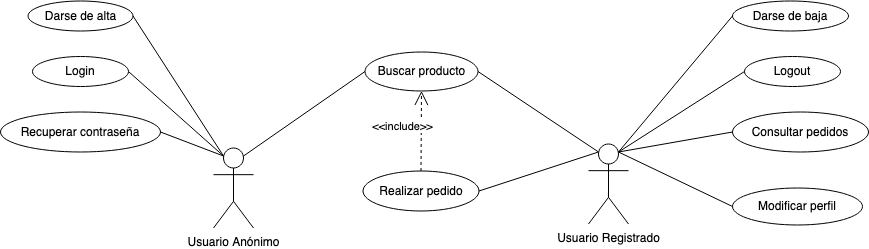
\includegraphics[width=\textwidth]{Use-Case_Diagram}
            \end{figure}

            \subsubsection{CU01\_Búsqueda}
            Proceso por el cual un usuario explora el cat\'alogo y acaba por visualizar la pagina de un libro.
            \begin{itemize}
                \item[+] Actores implicados: Usuario An\'onimo, Usuario Registrado.
                \item[+] Precondiciones: Nos encontramos en cualquiera de las p\'aginas que dan acceso al cat\'alogo.
                \item[+] Flujo principal:
                \begin{enumerate}
                    \item[1.] El usuario hace click en alguna de las categor\'\i{}as principales mostradas a modo de cat\'alogo flotante en la barra de navegacion
                    o hace click en \emph{All Books}.
                    \item[2.] El sistema muestra la p\'agina de resultados de b\'usqueda.
                    \item[3.] El usuario hace click en alguno de los productos mostrados.
                    \item[4.] El sistema muestra la p\'agina del libro.
                \end{enumerate}
                \item[+] Flujo alternativo: \emph{refinamiento\_b\'usqueda}. El usuario altera en la p\'agina de resultados alg\'un criterio de filtro.
                \begin{itemize}
                    \item[3.b.] El usuario selecciona/deselecciona alg\'un criterio de filtro de entre los mostrados en la p\'agina de resultados de b\'usqueda.
                    \item[4.b.] El sistema vuelve al punto 2 del flujo principal.
                \end{itemize}
                \item[+] Flujo alternativo: \emph{b\'usqueda\_por\_texto}. El usuario introduce una cadena de texto en el cuadro de b\'usqueda.
                \begin{itemize}
                    \item[1.b.] El usuario introduce una cadena de texto en el cuadro de b\'usqueda y hace click.
                \end{itemize}
            \end{itemize}

            \subsubsection{CU02\_Alta}
            Proceso por el cual se crea un nuevo usuario registrado.
            \begin{itemize}
                \item[+] Actores implicados: Usuario An\'onimo.
                \item[+] Flujo principal:
                \begin{enumerate}
                    \item[1.] El usuario hace click en el link de nuevo registro, disponible en la p\'agina de \emph{login}.
                    \item[2.] El sistema presenta un formulario donde introducir la direcci\'on de e-mail y la contrase\~na.
                    \item[3.] El usuario introduce y env\'\i{}a la informaci\'on pedida.
                    \item[4.] El sistema comprueba la informaci\'on proporcionada.
                    \item[5.] El sistema crea una nueva cuenta de usuario, pero la mantiene inactiva a la espera de confirmar la direcci\'on de email.
                    \item[6.] El sistema env\'\i{}a un email con un link de confirmaci\'on a la direcci\'on proporcionada, e informa al usuario por pantalla.
                    \item[7.] El usuario accede a su e-mail y hace click en el link enviado, confirmando que la direcci\'on de email es suya.
                    \item[8.] El sistema activa la cuenta de usuario.
                    \item[9.] El sistema env\'\i{}a al usuario un email de bienvenida.
                    \item[10.] El sistema redirige al usuario a la p\'agina de \emph{login}.
                \end{enumerate}
                \item[+] Flujo alternativo: \emph{usuario\_ya\_registrado}. La direcci\'on proporcionada se encuentra registrada en el sistema.
                \begin{itemize}
                    \item[5.b.] El sistema no crea una nueva cuenta de usuario.
                    Por razones de seguridad, la manera en que el sistema informa al usuario tras esta situacion es indistinguible del flujo principal,
                    de forma que no se pueda deducir que ese email ya tiene cuenta asociada en el sistema.
                \end{itemize}
                \item[+] Flujo alternativo: \emph{link\_ya\_enviado}. El sistema est\'a a la espera de la confirmacion de un link valido en esta direccion de email.
                \begin{itemize}
                    \item[5.b.] El sistema no crea una nueva cuenta de usuario. Se informa al usuario acerca de una condicion de error \-{}generica, por seguridad\- en relacion
                    con la direccion de email proporcionada, pidiendose que compruebe su direcci\'on de email.
                \end{itemize}
                \item[+] Flujo excepcional: \emph{time\_out}. El usuario no confirma su direccion de e-mail dentro de un plazo determinado.
                \begin{itemize}
                    \item[7.b.] El sistema detecta el timeout e invalida el link de confirmacion enviado. Si el usuario hace click en el link caducado se le informara de dicha condicion.
                \end{itemize}
            \end{itemize}

            \subsubsection{CU03\_Login}
                Proceso por el cual un usuario se autentica en el sistema.
                \begin{itemize}
                    \item[+] Actores implicados: Usuario An\'onimo.
                    \item[+] Flujo principal:
                    \begin{enumerate}
                        \item[1.] El usuario hace click en el link de \emph{login}, o intenta realizar alguna operaci\'on
                        que requiera autenticaci\'on (por ejemplo, a\~nadir un libro al carrito).
                        \item[2.] El sistema presenta el formulario de acceso (direcci\'on de email y la contrase\~na).
                        \item[3.] El usuario introduce y env\'\i{}a la informaci\'on pedida.
                        \item[4.] El sistema comprueba las credenciales.
                        \item[5.] El sistema redirige al usuario a la p\'agina principal.
                    \end{enumerate}
                    \item[+] Flujo alternativo: \emph{fallo\_autenticaci\'on}. El email no se encuentra registrado en el sistema, o la contrase\~na proporcionada no es correcta.
                    \begin{itemize}
                        \item[5.b.] El sistema informa al usuario acerca de un fallo gen\'erico de autenticaci\'on, de forma que,
                        por razones de seguridad, no se pueda deducir si el email proporcionado se encuentra registrado en el sistema.
                    \end{itemize}
                    \item[+] Flujo alternativo: \emph{bloqueo\_cuenta}. El usuario an\'onimo realiza, dentro de un marco de tiempo (configurable), un n\'umero de intentos (configurable) de login con contrase\~na err\'onea.
                    \begin{itemize}
                        \item[5.b.] El sistema bloquea la cuenta asociada al email para prevenir ataques por fuerza bruta.
                        \item[6.] El sistema informa al usuario por pantalla y mediante el env\'\i{}o de un email.
                        \item[7.] Pasado el tiempo de seguridad (configurable), el sistema desbloquea la cuenta del usuario.
                    \end{itemize}
                    \item[+] Post-Condiciones: El usuario pasa a tener rol de usuario registrado en el sistema.
                \end{itemize}

            \subsubsection{CU04\_RecuperarContrase\~na}
                Un usuario previamente registrado en el sistema intenta acceder al mismo, pero no recuerda su contrase\~na. El sistema intentar\'a crear una nueva contrase\~na y enviarla al e-mail del usuario.
                \begin{itemize}
                    \item[+] Actores implicados: Usuario An\'onimo.
                    \item[+] Flujo principal:
                    \begin{enumerate}
                        \item El usuario hace click en la opci\'on \emph{?`olvid\'o su contrase\~na?}.
                        \item El sistema presenta un formulario donde introducir la direcci\'on de e-mail.
                        \item El usuario introduce y env\'ia su direcci\'on de e-mail.
                        \item El sistema comprueba la direcci\'on de e-mail.
                        \item Comprobaci\'on correcta. El sistema env\'ia un e-mail con un link de confirmaci\'on a la direcci\'on proporcionada, e informa de ello al usuario por pantalla.
                        \item Link no caducado. El usuario accede a su e-mail y hace click en el link, confirmando que efectivamente la direcci\'on proporcionada es la suya.
                        \item El sistema genera una nueva contrase\~na y se la asigna al usuario.
                        \item El sistema env\'ia la nueva contrase\~na a la direcci\'on de e-mail del usuario, y le avisa de ello por pantalla.
                    \end{enumerate}
                    \item[+] Flujo alternativo: \emph{usuario\_no\_registrado}. La direccion proporcionada no se encuentra registrada en el sistema.
                    \begin{itemize}
                        \item[5.b.] El sistema no envia correo alguno pero, por razones de seguridad, desde el punto de vista del usuario este flujo alternativo es indistinguible del proncipal.
                    \end{itemize}
                    \item[+] Flujo excepcional: \emph{time\_out}. El usuario no confirma su direccion de e-mail dentro de un plazo determinado.
                    \begin{itemize}
                        \item[6.b.] El sistema detecta el timeout e invalida el link de confirmacion enviado. Si el usuario hace click en el link caducado se le informara de dicha condicion.
                    \end{itemize}
                \end{itemize}

            \subsubsection{CU05\_EditarPerfil}
                Proceso por el cual un usuario modifica alguno de los datos de su perfil personal.
                \begin{itemize}
                    \item[+] Actores implicados: Usuario Registrado.
                    \item[+] Flujo principal:
                    \begin{enumerate}
                        \item[1.] El usuario hace click en \emph{area personal}.
                        \item[2.] El sistema muestra la pagina de area personal, en donde se muestra el formulario de datos personales, rellenado con la informacion actual del usuario.
                        \item[3.] El usuario modifica los datos del formulario y lo envia al sistema.
                        \item[4.] El sistema comprueba los datos.
                        \item[5.] Comprobación correcta.El sistema actualiza la información del usuario.
                        \item[6.] El sistema muestra la pagina de inicio.
                    \end{enumerate}
                    \item[+] Flujo alternativo: \emph{error\_datos\_formulario}. Los datos proporcionados en el formulario de informacion personal no son validos.
                    \begin{itemize}
                        \item[5.b.] El sistema regresa al punto 3 del flujo principal, e informa al usuario acerca del fallo producido.
                    \end{itemize}
                    \item[+] Flujo alternativo: \emph{cancelar}. El usuario cancela el proceso de edicion de su informacion personal.
                    \begin{itemize}
                        \item[3.b.] El usuario hace click en el boton \emph{cancelar}. El sistema muestra la pagina de inicio.
                    \end{itemize}
                    \item[+] Post-Condiciones: El usuario ha alterado su informacion personal almacenada en la aplicacion.
                \end{itemize}

            \subsubsection{CU06\_RealizarPedido}
                Proceso por el cual un usuario realiza una compra a traves de la aplicacion web.
                \begin{itemize}
                    \item[+] Actores implicados: Usuario Registrado.
                    \item[+] Precondiciones: Desde cualquier pagina en la que se muestren libros (pagina de inicio, pagina de resultados de busqueda o pagina de un libro) el usuario hace click en \emph{add to cart}, para uno o mas libros.
                    \item[+] Flujo principal:
                    \begin{enumerate}
                        \item[1.] El usuario hace click en el icono del carrito.
                        \item[2.] El sistema muestra la pagina del carrito del usuario, con todos los libros contenidos en el mismo.
                        \item[3.] El usuario puede aumentar o disminuir el numero de unidades de un libro, o incluso eliminarlo por completo, y hace click en \emph{checkout}.
                        \item[4.] El sistema comprueba la disponibilidad de los libros contenidos en el carrito.
                        \item[5.] Stock suficiente. El sistema muestra la pagina de checkout, con el formulario de datos de envio y pago, y el resumen de la compra.
                        \item[6.] El usuario completa los datos de envio y de pago y hace click en \emph{Pay}.
                        \item[7.] El sistema tramita el pago.
                        \item[8.] Pago ok. El sistema registra el nuevo pedido.
                        \item[9.] El sistema confirma al usuario por pantalla y por e-mail que el pedido se ha realizado con exito.
                    \end{enumerate}
                    \item[+] Flujo alternativo: \emph{stock\_insuficiente}. No hay stock suficiente para satisfacer el contenido del carrito.
                    \begin{itemize}
                        \item[5.b.] El sistema vuelve al punto 2 del flujo principal, informando al usuario de los libros para los cuales no hay stock suficiente.
                        \item[3.b.] El usuario reduce la cantidad demandada de los libros correspondientes y hace click en \emph{checkout}.
                    \end{itemize}
                    \item[+] Flujo alternativo: \emph{error\_pago}. Error al efectuar el pago.
                    \begin{itemize}
                        \item[8.b.] El sistema vuelve al punto 5 del flujo principal, informando al usuario del problema respecto al pago.
                    \end{itemize}
                    \item[+] Flujo excepcional: \emph{libro\_eliminado}. Algun libro del carrito ya no esta disponible en el sistema.
                    \begin{itemize}
                        \item[5.b.] El sistema elimina del carrito automaticamente los libros que el administrador haya deshabilitado.
                        \item[6.b.] El sistema vuelve al punto 2 del flujo principal, informando al usuario de los libros que han sido eliminados.
                    \end{itemize}
                    \item[+] Post-Condiciones: El usuario ha efectuado un nuevo pedido.
                \end{itemize}

            \subsubsection{CU07\_ConsultarPedido}
                Proceso por el cual un usuario consulta el historial de pedidos que ha realizado.
                \begin{itemize}
                    \item[+] Actores implicados: Usuario Registrado.
                    \item[+] Flujo principal:
                    \begin{enumerate}
                        \item[1.] El usuario hace click en \emph{My Purchases} en la barra de navegacion.
                        \item[2.] El sistema muestra la pagina de los pedidos del usuario.
                        \item[3.] El usuario puede expandir-contraer la informacion mostrada relativa a un pedido.
                    \end{enumerate}
                \end{itemize}

            \subsubsection{CU08\_Baja}
                Proceso por el cual un usuario elimina su cuenta de la tienda online.
                \begin{itemize}
                    \item[+] Actores implicados: Usuario Registrado.
                    \item[+] Flujo principal:
                    \begin{enumerate}
                        \item[1.] El usuario hace click en \emph{area personal}.
                        \item[2.] El sistema muestra la pagina de area personal.
                        \item[3.] El usuario selecciona \emph{eliminar cuenta}.
                        \item[4.] El sistema muestra el formulario de eliminacion de cuenta.
                        \item[5.] El usuario completa y envia el formulario.
                        \item[6.] El sistema comprueba los datos.
                        \item[7.] Comprobacion correcta. El sistema actualiza el estado del usuario y envia un e-mail de confirmacion.
                        \item[8.] El sistema muestra la pagina de inicio.
                    \end{enumerate}
                    \item[+] Flujo alternativo: \emph{error\_datos\_formulario}. La contrase\~na proporcionada en el formulario de baja no es correcta.
                    \begin{itemize}
                        \item[7.b.] El sistema regresa al punto 4 del flujo principal, e informa al usuario acerca del fallo producido.
                    \end{itemize}
                    \item[+] Flujo alternativo: \emph{cancelar}. El usuario cancela el proceso de baja.
                    \begin{itemize}
                        \item[5.b.] El usuario cancela el proceso de baja. El sistema regresa al punto 2 del flujo principal.
                    \end{itemize}
                    \item[+] Post-Condiciones: El usuario ya no figura como dado de alta en la aplicacion.
                \end{itemize}

            \subsubsection{CU09\_Logout}
                Proceso por el cual un usuario cierra su sesi\'on en el sistema.
                \begin{itemize}
                    \item[+] Actores implicados: Usuario Registrado.
                    \item[+] Precondiciones: el usuario esta con su sesion abierta en el sistema.
                    \item[+] Flujo principal:
                    \begin{enumerate}
                        \item[1.] El usuario hace click en el link de \emph{logout}.
                        \item[2.] El sistema cierra la sesion del usuario.
                        \item[3.] El sistema muestra la pagina de inicio.
                    \end{enumerate}
                    \item[+] Post-Condiciones: El usuario ha efectuado el logout con exito.
                \end{itemize}


    % DISEÑO
    \section{Diseño}
    Dise
    \subsection{Arquitectura del Sistema}
    Arquitectura en capas. Capa de presentacion, capa de control, capa de servicio, capa de persistencia
    \subsection{Modelo de Datos}
    Modelo

    % IMPLEMENTACION
    \section{Implementacion}
    La implementacion del analisis y diseno detallados en los puntos anteriores lo conforma el conjunto de programas que se incluyen en el CD distribuido con la presente memoria.
    No obstante, en este apartado se ha querido comentar ciertos aspectos relevantes, que se pasan a explicar a continuacion.
    \subsection{Persistencia de Datos Jerarquicos. Categorias}
    \subsection{Validacion de Inputs}
    \subsubsection{ISBN}
    \subsection{Control de Concurrencia. Stock Consistente}
    \subsection{Creacion de Muestras}

    % TECNOLOGIAS
    \section{Stack Tecnol\'ogico}
    En este apartado se ofrece un comentario del stack tecnologico con el que se ha llevado a cabo la aplicacion web.

    \subsection{Spring Framework}
    \subsubsection{Spring Boot}
    \subsubsection{Spring MVC}
    \subsubsection{Spring Data JPA - Hibernate}
    \subsubsection{Spring Security}
    \subsection{Thymeleaf - HTML5}
    \subsection{Bootstrap 4 - CSS3}
    \subsection{Stripe}
    \subsection{PostgreSQL}
    \subsection{JavaScript}
    \subsubsection{Ajax}
    \subsection{FontAwesome - Pretty Checkbox - Google Fonts}
    \subsection{Tecnologias Transversales}
    \subsubsection{Git}
    \subsubsection{Java 11}
    \subsubsection{Maven}
    \subsubsection{IntelliJ IDEA}
    \subsubsection{Logback}
    \subsubsection{Lombok}
    \subsubsection{Guava}

    % DESPLIEGUE Y SEGURIDAD
    \section{Despliegue y Seguridad}
        \subsection{Heroku Platform}
            \subsubsection{Heroku-postgresql}
            \subsubsection{PaperTrail}
            \subsubsection{Snyk}
        \subsection{Spring Security}
        \subsection{HTTPS}
        \subsection{Cross-Site Request Forgery}
        \subsection{Brute-Force Authentication}

    % MANUALES
    \section{Manuales}
    En esta seccion se va a describir las cuestiones necesarias para facilitar el uso de la aplicacion web por parte de los usuarios
        \subsection{Usuario Cliente}
    aqui va la descripcion para el usuario cliente
        \subsection{Usuario Administrador}
    aquie se describe el uso del admin

    % MEJORAS Y AMPLIACIONES
    \section{Mejoras y Ampliaciones}
    Testar el software
    Sistema de valoracion por parte de los usuarios de los libros


\end{document}
